\subsection{Introducción}

En este punto vamos a aplicar la heurística de búsqueda local para intentar mejorar la solución a partir de una solución particular, vamos a mostrar cómo armamos los conjuntos de vecindades y cómo aplicamos el algoritmo para descubrir una solución mejor a la solución que teníamos inicialmente.

La idea básica de los algoritmos de búsqueda local es la siguiente, en general la idea siempre es la misma:

\begin{itemize}
  \item Iniciar con una solución generada aleatoriamente o hallada con algún otro algoritmo.
  \item Aplicar a la solución actual una transformación de algún conjunto dado de transformaciones para mejorar la solución (vecindades).
  \item La solución mejorada se convierte en la solución actual, repetir hasta que ninguna transformación del conjunto mejore a la solución actual.
\end{itemize}

En nuestro caso, vamos a utilizar esta idea, pero para ello es necesario que nos definamos estas trasformaciones y podamos asi compararla con la solución inicial de la cual partimos.

En la figura \ref{fig: ej3_ejemplo_mejora} podemos ver un ejemplo de cómo el algoritmo de búsqueda local va mejorando la solución en función de las iteraciones del ciclo (épocas).

\begin{figure}[H]
  \begin{center}
    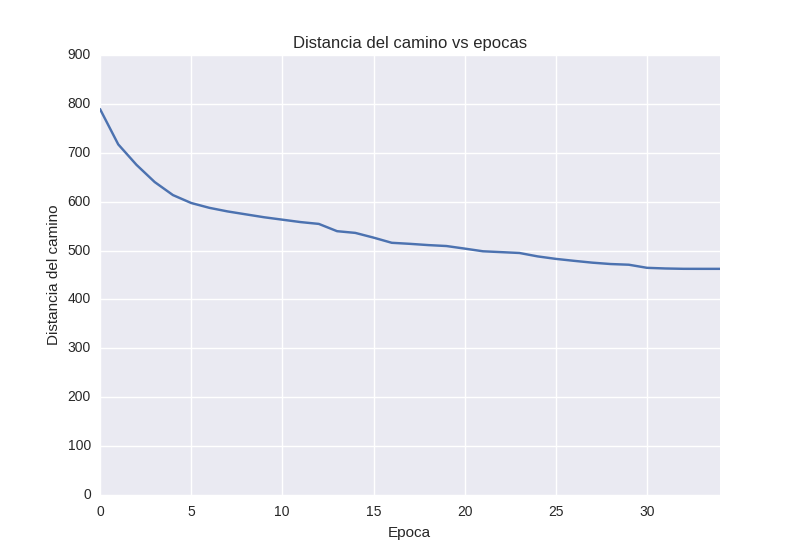
\includegraphics[width=\textwidth]{img/ejercicio3/ejemplo_cambios.png}
    \caption{Ejemplo del funcionamiento de la heurística de búsqueda local.}
    \label{fig: ej3_ejemplo_mejora}
  \end{center}
\end{figure}

\subsection{Explicación de la heurística de búsqueda local}
\label{sec: ej3_explicacion}

Para esta heurística presentamos 4 tipos de vecindades distintas, esto nos permite poder intentar mejorar una solución inicial. En nuestro caso comenzamos con un goloso, y vamos construyendo las distintas vecindades, luego elegimos alguna de ellas y buscamos la mejor solución que mejore la inicial.

\begin{itemize}

\item La primer vecindad va a estar compuesta por todas las soluciones que surjan de cambiar las pokeparadas que quedaron fuera de la solución con las que están dentro de la solución inicial, entonces por cada una de las paradas de la solución vamos a ir haciendo swap con una de las paradas que quedaron fuera, como estamos haciendo el cambio entre paradas no hace falta que revisemos si el camino resultante es válido.

\item La segunda está compuesta por las pokeparadas de la solución, es decir, vamos a ir intercambiando el orden de estas paradas dentro de la solución.

\item La tercera involucra a gimnasios y a pokeparadas, en esta vamos a ir intercambiando el orden de visita tanto de pokeparadas como de gimnasios, para ellos vamos a ir recorriendo la solución de principio a fin e intercambiando una pokeparada/gimnasio con el siguiente.

\item La última vecindad que planteamos se trata de intercambiar las posiciones de los gimnasios dentro de la solución, para ellos necesitamos que sea válido para tomarlo con un vecino posible.

\end{itemize}

En la primer vecindad, comenzamos por obtener una solución de una instancia por medio del algoritmo goloso. Partiendo de esta base, vamos a intentar intercambiar las paradas de esta solución con las pokeparadas que quedaron afuera y no son parte de la solución que devolvió el goloso. Para poder recorrer todas las pokeparadas dentro de la solución e ir intercambiandolas con las de afuera, tuvimos que quedarnos con las pokeparadas iniciales.
Esto nos permite poder saber rápidamente cuáles son las que no pertecen a la solución. Entonces, por cada una de las pokeparadas de la solución vamos a ir intercambiándola con alguna parada que quedó fuera, luego vamos a calcular la distancia total otra vez y compararla con la distancia total anterior (es decir, antes de que hagamos el intercambio de paradas) para quedarnos con alguna mejor.

Para la segunda vecindad, fuimos recorriendo cada pokeparada de la solución e intercambiándola con otra parada de la misma solución pero que se encuentre por delante, es decir como la solución viene ordenada para representar el camino, vamos a querer cambiar las paradas futuras y así establecer otro orden de visita de las mismas. Es por ello que cada vez que querramos intercambiar pokeparadas nos aseguramos que sean paradas de la solución y no gimnasios.

Para la tercera vecindad, lo único que tuvimos que hacer es recorrer la solución desde el principio al final e intercambiar los nodos. Cada nodo de la solución lo cambiamos con el siguiente y preguntamos si era una solución válida. Si era válida, entonces nos la guardamos.

La última vecindad lo que hacemos es intercambiar los gimnasios dentro de la misma solución entre ellos, para ello recorremos la solución y vamos intercambiando cada uno con los siguientes. Luego de cada cambio, verificamos si la solución es válida. En caso positivo, la guardamos. Luego, se vuelve el cambio atrás para continuar con otro cambio.


La búsqueda local en sí, se hace a partir de estas vecindades, en nuestro algoritmo tenemos una entrada que indica el tipo de vecindades que va a utilizar.
Esta entrada es de longitud 4 y se espera que este compuesta por algún '1' en el caso que se quiera hacer la búsqueda usando una vecindad. Pasamos a detallarlo mejor a continuación.
\begin{itemize}
\item entrada = '1xxx' Este tipo de entrada lo que indica es que se va hacer la búsqueda usando una sola vecindad, dicha vecindad es la primera que se indica más arriba.

\item entrada = 'x1xx' Este tipo de entrada indica que se hará la búsqueda sólo con la segunda vecindad.

\item entrada = 'xx1x' Se hará la búsqueda con la tercera vecindad.

\item entrada = 'xxx1' se hará la búsqueda con la cuarta vecindad.
\end{itemize}

Además de esto, también podemos combinar vecindades o utilizar todas. En el caso de utilizar todas, la entrada sería '1111'.
Lo que hacemos básicamente es observar qué vecindad o qué vecindades se indicaron para hacer la búsqueda, obtener todas esas soluciones vecinas y comparar cuál de ellas es la mejor y devolverla.

\subsection{Cota de complejidad}

Para el cálculo de complejidad vamos a usar siempre N, como cantidad de elementos totales de una instancia del problema, es decir, la suma de pokeparadas y gimnasios.

\subsubsection{Análisis de las vecindades}

\begin{itemize}

\item  Vecindad con las pokeparadas de los de afuera:

\begin{verbatim}
pokeNueva = 0;
pokeVieja = 0;
 Por cada N nodo en la solución
  Si N es una pokeparada 
   Por cada M nodo en las pokeparadas totales del la instancia
    Si M no esta en la solución
     Pokenueva = M;
     PokeVieja = N;
     Intercambio N por M en la solución nueva
     Me guardo en RESULTADO la solución que acabo de encontrar.
     Reestablezco la solución intercambiando M por N  
return RESULTADO;
\end{verbatim}

Al recorrer todos los nodos de la solución inicial tenemos un complejidad lineal en la cantidad de nodos de dicha solución$ O(N)$. Luego, por cada nodo de estos, necesitamos ver si es una pokeparada, lo cual se puede hacer de forma inmediata, ya que solo es ver que el valor del nodo sea menor a la cantidad de gimnasios totales, eso es $O(1)$. Luego iteramos por cada N (en el pseudocodigo) los M, que es un elemento del conjunto de las pokeparadas totales de la instancia. Por esta iteracion tenemos $O(N)$ en peor caso, donde N es la cantidad total de nodos de una instancia, pero luego como lo estamos haciendo para cada N, este doble ciclo tiene una complejidad de $O(N^2)$. Por ultimo, necesitamos también averiguar si la nueva solución que nos creamos al intercambiar dos paradas es válida, para ello tenemos que recorrer linealmente cada nodo y ver si existen suficientes paradas para derrotar al gimnasio próximo que se lista en la solución, esto tiene un costo de $O(N)$ en la cantidad de nodos totales, luego tenemos asignaciones, intercambios y un push de la solución a un acumulador de soluciones.
Finalmente la complejidad de nuestro calculo de esta vecindad es $O(N^3)$ en peor caso.

\item Vecindad con las pokeparadas de las de adentro:

\begin{verbatim}
 Por cada N nodo en la solución
  Si N es una pokeparada 
   busco nodos (M) desde la posicion de N en adelante en la solución
    Si M es pokeparada
     Intercambio N con M en la solución.
      Si esta solución nueva es válida
       Me guardo en RESULTADO la solución que acabo de encontrar.
      Reestablezco la solución intercambiando M por N  
return RESULTADO;
\end{verbatim}

En sí es muy parecida al vecindario anterior. Se recorre cada nodo de la solución en tiempo lineal $O(N)$ y por cada uno de estos, necesito averiguar si es pokeparada $O(1)$ y por cada N vamos a recorrer M nodos, estos M nodos son los nodos siguientes de la solución, acotando groseramente podemos decir que tiene un orden de $O(N)$, haciendo que esos dos ciclos anidados cuesten $O(N^2)$, por último necesitamos hacer un swap $O(1)$ y averiguar si la solución que encontramos es válida, por lo explicado mas arriba, esto tiene un costo de $O(N)$.
En resumen el costo calculado de esta vecindad es $ O(N^3)$.

\item Vecindad cambiando solo los adyacentes de a dos:
\begin{verbatim} 
 Por cada N nodo en la solución 
  Intercambio N con N+1 en la solución.
   Si esta solución nueva es válida
    Me guardo en RESULTADO la solución que acabo de encontrar.
   Reestablezco la solución intercambiando N+1 por N  
return RESULTADO;
\end{verbatim}

En este vecindario calculamos aquellas soluciones que se obtienen cambiado el orden de alguna pokeparada o gimnasio con otra pokeparada o gimnasio, siempre recorriendo hacia adelante.
Para ellos vamos a recorrer todos los nodos de la solución e iremos intercambiando ese nodo con el siguiente. esto lo hacemos en $O(N)$. Luego, necesitamos verificar si la solución tras intercambiar dos nodos adyacentes es válida. Eso tambien tiene un costo lineal en la cantidad de nodos ($O(N)$). Luego hace algunas asignaciones y reestablece la posición del nodo swapeado, con lo cual la complejidad del calcula de esta vecindad es $O(N^2)$.

\item Vecindad cambiando la posición de los gimnasios:
\begin{verbatim} 
 Por cada N nodo en la solución
  Si N no es una pokeparada 
   busco nodos (M) desde la posicion de N en adelante en la solución
    Si M no es pokeparada
     Intercambio N con M en la solución.
      Si esta solución nueva es válida
       Me guardo en RESULTADO la solución que acabo de encontrar.
      Reestablezco la solución intercambiando M por N  
return RESULTADO;
\end{verbatim}

Y por último el vecindario que cambia los gimnasios de lugar dentro de la solución, tiene la misma complejidad temporal que la segunda vecindad, donde cambiábamos las pokeparadas de adentro de la solución. Luego la complejidad temporal es $ O(N^3)$.

\end{itemize}

Como podemos ver todas las vecindades propuestas son de costo polinomial con respecto a la cantidad de nodos.

\subsubsection{Análisis de la complejidad total}

A continuación vamos a enunciar un pseudocódigo del algoritmo completo para luego analizarlo y sacar conclusiones sobre la complejidad total.

\begin{algorithm}[H]
  \label{algo: ej3_pseudocodigo}
  \BlankLine

  $solucion \gets $algoritmo\_goloso()\\
  $cambio \gets true$\\
  $repeticiones \gets 0$\\
  \While{$cambio \wedge repeticiones < \#nodos$}{
    \BlankLine

    $cambio \gets false$\\
    $vecindades \gets $calcular\_vecindades()\\
    $vecina \gets $vecina con minima distancia de $vecindades$\\

    \BlankLine
    \If{ distancia($vecina$) $<$ distancia($solucion$) }{
      \BlankLine
      
      $solucion \gets vecina$\\
      $cambio \gets true$
      
      \BlankLine
    }

    \BlankLine
  }


  \BlankLine
  \caption{Pseudocódigo del algoritmo de búsqueda local.}
\end{algorithm}

\medskip

Veamos más en detalle las partes importantes del algoritmo:

\begin{itemize}
  \item En la linea 1 se llama a una implementación de un algoritmo goloso que nos da una primera solución al problema. Esto, como vimos en el ejercicio 2 (Sección \ref{sec: ej2_cota}) es del orden O(\textit{max}($m^2, n^2, m*n$)).
  \item En la linea 6 se calculan las vecindades. Como vimos en la subsección previa, esto es O($N^3$) para cualquiera de las vecindades.
  \item En la linea 7 se busca el mínimo de las vecindades obtenidas. Cómo calcular las vecindades es O($N^3$) sabemos que iterarlas debe costar menos.
  \item En la guarda del if de la linea 8 se calculan las distancias de los caminos. A lo sumo un camino puede contener todo los nodos, entonces recorrerlo es O($N$).
  \item En la linea 9 se copia el camino, lo cual es iterar entre todos los nodos y copiar un número (el índice). Por esto es O($N$).
  \item El ciclo general, con su guarda en la linea 4 itera mientras se mejore la solución. Pero también existe una cota superior: la cantidad de repeticiones. Lo que hace el algoritmo es no entrar al ciclo más de $N$ veces. Por ende, lo que está en el ciclo se repite a los sumo $N$ veces.
\end{itemize} 

Teniendo en cuenta los puntos planteados, podemos ver que el algoritmo itera en el ciclo a lo sumo $N$ veces. También sabemos que el cuerpo del ciclo cuesta O(\textit{max}($m^2, n^2$) + $N^3$ + $N$). Veamos en detalle esta cota:

\begin{equation}
  max(m^2, n^2) + N^3 + N = max(m^2, n^2) + (m+n)^3 + m + n
\end{equation}
Analicemos la parte de la derecha
\begin{equation}
  (m+n)^3 + m + n = m^3 + 3m^2n + 3mn^2 + n^3 + m + n
\end{equation}
Ahora volvamos a ver toda la cota completa:
\begin{equation}
  O( max(m^2, n^2) + m^3 + 3m^2n + 3mn^2 + n^3 + m + n )
\end{equation}
Como sabemos que $n > 0$ y $m > 0$ podemos acotarlo por:
\begin{equation}
  O( max(m^3, n^3) )
\end{equation}

Tenemos entonces que la complejidad del cuerpo es del orden O($max(m^3, n^3)$). Teniendo en cuenta la cota de iteraciones del ciclo, podemos decir que la complejidad total es O($N * max(m^3, n^3)$).

Veamos más en detalle este valor:
\begin{equation}
  N * max(m^3, n^3) = (m+n) * max(m^3, n^3)
\end{equation}
Tenemos tres posibles casos:
\begin{equation}
  si\ m > n \Rightarrow max(m^3, n^3) = m^3 \Rightarrow (m+n) * max(m^3, n^3) <= m^4
\end{equation}
\begin{equation}
  si\ m < n \Rightarrow max(m^3, n^3) = n^3 \Rightarrow (m+n) * max(m^3, n^3) <= n^4
\end{equation}
\begin{equation}
  si\ m = n \Rightarrow max(m^3, n^3) = n^3 = m^3 \Rightarrow (m+n) * max(m^3, n^3) <= n^4 = m^4
\end{equation}
Entonces nos queda que
\begin{equation}
  O(N * max(m^3, n^3)) = O(max(m^4, n^4))
\end{equation}

Por lo tanto, podemos decir que la complejidad del algoritmo es del orden \textbf{O($\boldsymbol{max(m^4, n^4)}$)}.

\subsection{Experimentación}

\par Como mencionamos previamente, se implementaron distintos tipos de vecindades. Creímos importante poder comparar estas versiones y ver para cada caso si agregar un tipo de vecindad beneficia o simplemente empeora los tiempos de ejecución. Generamos distintas versiones del programa con un formato característica que se explica detalladamente en la sección \ref{sec: ej3_explicacion}.

\par A continuación vamos a analizar el desempeño de las distintas versiones de vecindades implementadas.

\subsubsection{Experimento 1: Cantidad de paradas vs Tiempos de ejecución}

\par Para el primer experimento vamos a variar la cantidad de paradas y ver como se comportan las distintas vecindades con respecto a los tiempos de ejecución. Vamos a fijar los parámetros \textit{cantidad de gimnasios = 5} y \textit{capacidad de la mochila = 5} y aumentar \textit{cantidad de paradas} desde 2 hasta 999.

\par Creemos que los tiempos de ejcución de las versiones con más vecindades van a ser claramente mayoes con respecto a las otras. Porque las vecindades se basan en cambios de nodos y al ir aumentando la cantidad de paradas se generan mucha cantidad de combincaciones tornandose muy pesado (en cuanto a procesamiento).

\begin{figure}[H]
  \begin{center}
    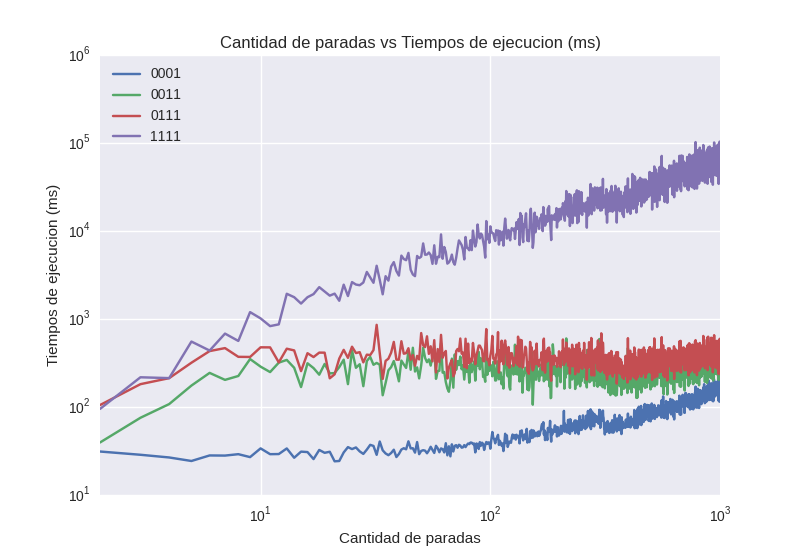
\includegraphics[width=\textwidth]{img/ejercicio3/exp1.png}
    \caption{Resultados del experimento 1.}
    \label{fig: ej3_exp1}
  \end{center}
\end{figure}

\par En la figura \ref{fig: ej3_exp1} podemos ver los resultados del experimento 1. Como esperábamos, vemos que las versiones con más vecindades conllevan mucho más tiempo de ejecución. Pero esto se verá reflejado en la calidad de la solución, ya que al buscar entre más vecindades creemos que tendrá más posibilidades de acercarte a la solución.

\par Para los casos con mayor cantidad de paradas notamos una diferencia muy grande. Inclusive, la versión $1111$ (con todas las vecindades) parece tomar una complejidad del orden cuadrático (lineal en el gráfico, porque los ejes están en escala logarítmica).





\subsubsection{Experimento 2: Cantidad de gimnasios vs Tiempos de ejecución}

\par En este caso, vamos a variar la cantidad de gimnasios y seguiremos midiendo los tiempos de ejecución de las distintas vecindades. Para esto, fijamos los parámetros \textit{cantidad de paradas = 100} y \textit{capacidad de la mochila = 5} y aumentaremos \textit{cantidad de gimnasios} desde 2 hasta 80.

\par Luego de haber visto los resultados del experimento anterior, esperamos aquí también que las versiones con más vecindades sufran mucho estos cálculos y esto se vea reflejado en los tiempos de ejecución. Queremos ver si se dan resultados similares al experimento anterior o si las complejidades cambian.

\begin{figure}[H]
  \begin{center}
    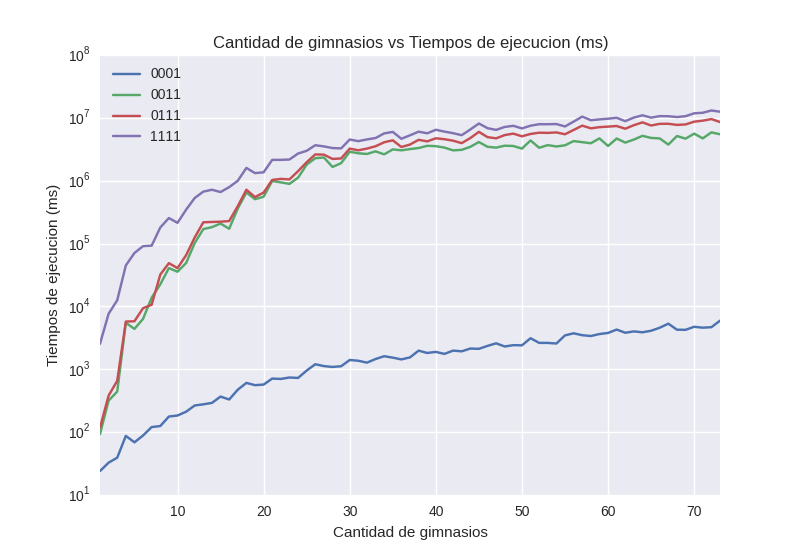
\includegraphics[width=\textwidth]{img/ejercicio3/exp2.png}
    \caption{Resultados del experimento 2.}
    \label{fig: ej3_exp2}
  \end{center}
\end{figure}

\par Con respecto al momento de ralizar la experimentación, debemos hacer un comentario. En un comienzo se había pensado en aumentar hasta la cantidad 300, pero se tuvo que limitar esta cantidad porque al ir aumentando los gimnasios se debe tomar \textit{cantidad de paradas} con un valor elevado y esto hizo que los tiempos de ejecución crecieran mucho más rápido. Luego de mucho tiempo de procesamiento, se debió frenar la experimentación en 80.

\par En la figura \ref{fig: ej3_exp2} podemos ver los resultados del experimento 2. Se nota claramente como la versión con solo un tipo de vecindad (0001) se ubica muy por debajo del resto. Lo que notamos también es que a partir de una cantidad elevada de gimnasios (aproximadamente 30) la diferencia entre las otras tres versiones se achica y se mantiene bastante estable. Esto creemos que es un punto a favor para utilizar la versión con más vecindades (1111), porque vemos que para casos más interesantes los tiempos de ejecución, con respecto a las versiones 0111 y 0011, no se diferencia tanto. Tendremos que tener en cuenta esto a la hora de comparar las versiones en función de la calidad de sus soluciones.



\subsubsection{Experimento 3: Calidad}

\par Luego de haber medido los tiempos de ejecución, creemos necesario comparar los resultados obtenidos entre las distintas versiones para poder luego, con los experimentos realizados, determinar qué versión será la definitiva.

\par Para comparar las soluciones que nos brinda cada versión correremos una serie de casos de distintos tipos y analizaremos los datos obtenidos. Estos casos van a ser generados de la siguiente forma:

\begin{itemize}
  \item para el parámetro \textit{cantidad de gimnasios} se toma un valor de manera aleatoria entre 1 y 10.
  \item para el parámetro \textit{cantidad de paradas} se toma un valor de manera aleatoria entre 1 y 10.
  \item para el parámetro \textit{capcidad de la mochila} se toma un valor de manera aleatoria entre 1 y 7.
\end{itemize}

\par Se generaron 100 casos. Algunos de los casos generados resultaron ser inválidos (sin solución), ya que no queríamos dejar afuera estos casos, aunque para algunos análisis se los va a dejar de lado.

\par Se corrieron estos casos en las 4 versiones y en el algoritmo exacto. A partir de ahora analizaremos los resultados obtenidos.

\medskip

\textbf{Análisis 1: Porcentaje de error}

\par Lo primero que queremos ver en los resultados de la experimentación es qué tan cerca de la solución exacta estuvo cada versión del programa. Para esto, realizamos un procentaje de error en cada caso de entrada. Por ejemplo, si la solución exacta era $10$ y el programa nos dió $9$, hay un 10\% de error. Luego sacamos un promedio del procentaje de error de todos los casos agrupado por versión del programa y obtuvimos los datos que vemos en el cuadro \ref{tab: ej3_exp3_an1_prom}.

\newcolumntype{C}[1]{>{\centering\let\newline\\\arraybackslash\hspace{0pt}}m{#1}}

\begin{table}[!htb]
  \caption{Porcentajes de error por versión del programa}
  \label{tab: ej3_exp3_an1_prom}
  \begin{subtable}{.5\linewidth}
    \caption{Todos los casos.}
    \label{tab: ej3_exp3_an1_prom_todos}
    \centering
    \begin{tabular}{|C{0.5cm}|C{2cm}|C{2cm}|}
      \hline
      {} & Versión del programa &  Porcentaje de error \\
      \hline
      0 &             '0001' &            69.13\\
      1 &             '0011' &            50.13\\
      2 &             '0111' &            34.45\\
      3 &             '1111' &            30.14\\
      \hline
    \end{tabular}
  \end{subtable}
  \begin{subtable}{.5\linewidth}
    \centering
    \caption{Casos con solución válida.}
    \label{tab: ej3_exp3_an1_prom_validados}
    \begin{tabular}{|C{0.5cm}|C{2cm}|C{2cm}|}
      \hline
      {} & Versión del programa &  Porcentaje de error \\
      \hline
      0 &             '0001' &            73.93\\
      1 &             '0011' &            53.61\\
      2 &             '0111' &            36.84\\
      3 &             '1111' &            32.23\\
      \hline
    \end{tabular}
  \end{subtable}
\end{table}

\par En ambos cuadros podemos ver que el procentaje de error va disminuyendo a medida que se aplican más tipos de vecindad. Esto era de esperarse. Pero lo que nos sorprende es la magnitud de las diferencias. Por ejemplo, en el cuadro \ref{tab: ej3_exp3_an1_prom_validados} vemos que la versión $0011$ tiene un procentaje de error del 50.47\%. Consideramos este valor como una aproximación muy burda de la solución, ya que estaría haciendo recorrer un 50\% más de distancia. En cambio las versiones $0111$ y $1111$ tiene un procentaje cercano al 30\%. Esta cota si nos parece un poco más acertada, pero queremos ver más en detalle cómo se distribuyen esos errores. Porque, por ejemplo, que el promedio de la versión $1111$ sea el 30.14\% nos da una idea, pero no sabemos si hay alguna solución muy lejana que nos esté influenciando mucho y tal vez separando un par de casos particulares podemos obtener un promedio mejor.

\par Para analizar mejor estos valores vamos a ver cómo se distribuyen estos porcentajes de error. Nos vamos a enfocar únicamente en los casos con solución válida.

\begin{figure}[H]
  \begin{center}
    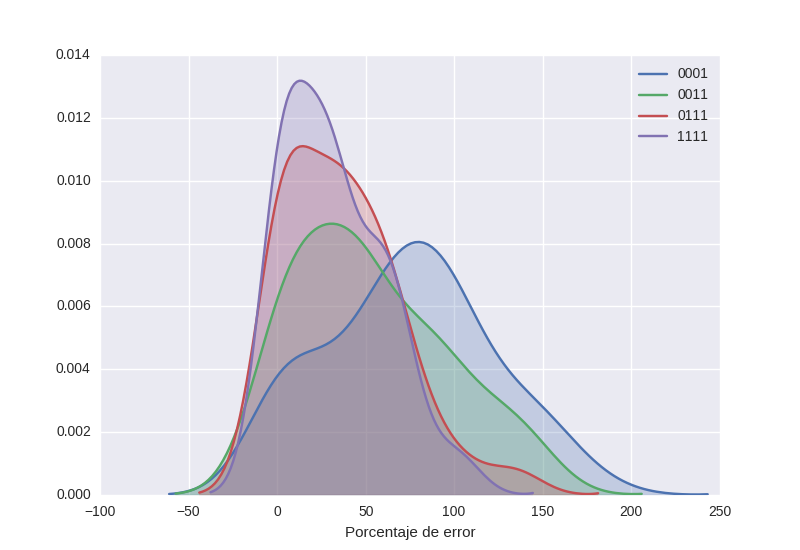
\includegraphics[width=\textwidth]{img/ejercicio3/exp3_distribuciones.png}
    \caption{Distribución de los porcentajes de error sobre casos con solución válida.}
    \label{fig: ej3_exp3_an1_distr_validados}
  \end{center}
\end{figure}

\par Podemos ver en la figura \ref{fig: ej3_exp3_an1_distr_validados} cómo los porcentajes de error obtenidos por la versión $1111$ se mantienen en un rango acotado, siendo el promedio un valor bastante representativo de los resultados en general. Esto nos indica que podemos acercanos en un 30\% a la solución exacta del problema con una probabilidad grande. Mientras que por ejemplo la versión $0111$ presenta una amplitud de porcentajes mayor, lo que nos indica que podemos obtener un resultado cercano al 30\%, pero que también tenemos una probabilidad (menor, pero no despreciable) de obtener un resultado que se diferencie en un 50\% y hasta 100\% de la solución exacta.



\subsubsection{Experimento 4: Cota del ciclo}

\par En este último experimento, queremos poner a prueba la cota máxima de iteraciones que le impusimos al ciclo del algoritmo. Hasta el momento solo la mencionamos. Por esto, queremos correr una cantidad importante de casos aleatorios para ver qué cantidad de veces ingresan al ciclo y analizar así si la cota impuesta es buena o si estamos perdiendo calidad saliendo antes del ciclo.

\par Para lleva a cabo el experimento, generamos una serie de casos random aumentando la cantidad de nodos desde 2 hasta 500. Para cada cantidad generamos varios casos. Luego, correremos estos casos sobre la versión $1111$ y contaremos la cantidad de veces que ingresa al ciclo.

\begin{figure}[H]
  \begin{center}
    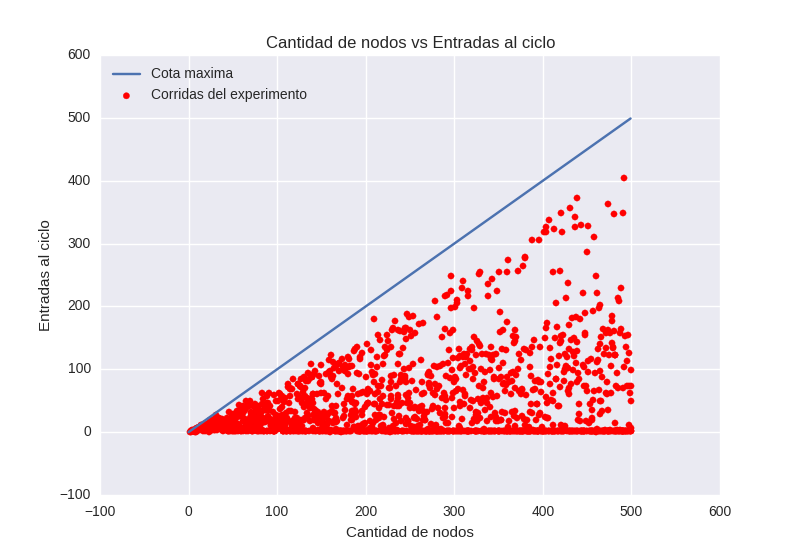
\includegraphics[width=\textwidth]{img/ejercicio3/exp4.png}
    \caption{Resultados del experimento 4.}
    \label{fig: ej3_exp4}
  \end{center}
\end{figure}

\par En la figura \ref{fig: ej3_exp4} podemos ver los resultados del experimento. La linea en azul indica la cota implementada, mientras que los puntos rojos son los datos obtenidos de las corridas. Notamos que la cantidad de entradas al ciclo se mantiene por debajo de la cota, lo que nos indica que la cota no nos está privando de mejores soluciones, sino que el algoritmo sale del ciclo (porque no logra mejorar la solución) antes de llegar a la cota. Solo en los casos con cantidad de nodos muy pequeña vemos que llega a la cota, pero a partir de aproximadamente 30 nodos la cota deja de influir.

\par Podemos concluir así que la cota tomada es buena y parece comportarse correctamente. No podemos asegurar que esto ocurra para todos los casos posibles, pero consideramos que la cota se comporta bien para una buena cantidad y vamos a dejarla.



\bigskip

\par Concluimos que la mejor versión es la que utiliza todas las vecindades ($1111$). A pesar de que nos hubiera gustado indagar más profundo en cuanto a la relación calidad-tiempo, creemos que los tiempos de ejecución no son tan elevados en los casos generales. En cuanto a calidad, nos quedamos claramente con las versiones $0111$ y $1111$. En cuanto a tiempos, vimos que para algunos casos había una gran diferencia y para otros no. Por esto nos quedamos con la versión que nos asegura mejora calidad y correremos los riesgos de tener casos con tiempos de ejecución elevados. más adelante (en el ejercicio 5) podremos ver si esta decisión fue acertada o si los tiempos de ejecución castigan a este algoritmo y no le permiten competir fuertemente con los otros algoritmos.